\section{Sample Cases}


For the purposes of the computation, we simplify our cost functional and use the squared length instead of true length in \( L \) in order to accommodate the coding format. Even with this simplification, the model is robust and provides a reasonable representation of the trajectories. This is evidenced by the following four test cases: 

\begin{enumerate}
    \item Two robots with parallel destination.
    
    \item Two robots with paths that intersect.
    
    \item Two robots and one obstacle.
    
    \item Two or more robots with two or more obstacles.
    
\end{enumerate}

Below is our algorithm we used to test these cases (for the 2 robots and 1 obstacle case; more robots and obstacles cases are similar):
\begin{lstlisting}
    import numpy as np 
    import matplotlib.pyplot as plt
    import scipy.integrate as int
    # weights 
    # Repulsiveness between of robots
    C1 = 1
    # Repulsiveness of obstacles
    C2 = 3
    # Robots
    robot1_start = #insert initial position for robot 1
    robot1_end = #insert final position for robot 1
    robot2_start = #insert initial position for robot 2
    robot2_end = #insert final position for robot 2
    #
    # Obstacles
    obs1_radius = #specify size of radius of obstacle
    obs1_pos = #specify location of center of obstacle
    #
    robot1_x = #insert guess for x position for robot 1
    robot1_y = #insert guess for y position for robot 1
    robot2_x = #insert guess for x position for robot 2
    robot2_y = #insert guess for y position for robot 2
    #Model
    def dxydt(t, x_y):
    x1, y1, x2, y2, dx1, dy1, dx2, dy2 = x_y

    x1_el = -(C1 * (x1 - x2)) / ((x1 - x2) ** 2 + (y1 - y2) ** 2) ** 2 - C2 * (x1 - 2) 

    / (np.sqrt((x1 - obs1_pos[0]) ** 2 + (y1 - obs1_pos[1]) ** 2) - obs1_radius) ** 3 

    / np.sqrt((x1 - obs1_pos[0]) ** 2 + (y1 - obs1_pos[1]) ** 2)

    y1_el = -(C1 * (y1 - y2)) / ((x1 - x2) ** 2 + (y1 - y2) ** 2) ** 2 - C2 * (y1 - 2) 

    / (np.sqrt((x1 - obs1_pos[0]) ** 2 + (y1 - obs1_pos[1]) ** 2) - obs1_radius) ** 3 

    / np.sqrt((x1 - obs1_pos[0]) ** 2 + (y1 - obs1_pos[1]) ** 2)

    x2_el = (C1 * (x1 - x2)) / ((x1 - x2) ** 2 + (y1 - y2) ** 2) ** 2 - C2 * (x2 - 2) 

    / (np.sqrt((x2 - obs1_pos[0]) ** 2 + (y2 - obs1_pos[1]) ** 2) - obs1_radius) ** 3 

    how / np.sqrt((x2 - obs1_pos[0]) ** 2 + (y2 - obs1_pos[1]) ** 2)

    y2_el = (C1 * (y1 - y2)) / ((x1 - x2) ** 2 + (y1 - y2) ** 2) ** 2 - C2 * (y2 - 2) 

    / (np.sqrt((x2 - obs1_pos[0]) ** 2 + (y2 - obs1_pos[1]) ** 2) - obs1_radius) ** 3 

    / np.sqrt((x2 - obs1_pos[0]) ** 2 + (y2 - obs1_pos[1]) ** 2)

    return dx1, dy1, dx2, dy2, x1_el, y1_el, x2_el, y2_el


    # Boundary Conditions
    def bc(ya, yb):
    return ya[0] - robot1_start[0], yb[0] - robot1_end[0] , ya[1] - robot1_start[1]
    , yb[1] - robot1_end[1], ya[2] - robot2_start[0]
    , yb[2] - robot2_end[0], ya[3] - robot2_start[1], yb[3] - robot2_end[1]

    t_guess = np.linspace(0, 1, 5)
    xy_guess = np.zeros((8, t_guess.size))
    xy_guess[0] = robot1_x
    xy_guess[1] = robot1_y
    xy_guess[2] = robot2_x
    xy_guess[3] = robot2_y
    res = int.solve_bvp(dxydt, bc, t_guess, xy_guess)
\end{lstlisting}

In addition, we have the following code designed to test the cases we outlined in the beginning of this section.

\begin{lstlisting}
    #Plots for the paths of robots 1 and 2:

    t = np.linspace(0, 1, 201)
    obs_t = np.linspace(0, 2 * np.pi, 51)
    plt.plot(res.sol(t)[0], res.sol(t)[1], label = 'Robot 1')
    plt.plot(res.sol(t)[2], res.sol(t)[3], label = 'Robot 2')
    plt.plot(obs1_radius * np.cos(obs_t) + obs1_pos[0], obs1_radius * np.sin(obs_t)
         obs1_pos[1], label = 'obstacle')
    plt.legend()

    #Plots that verify collision free paths between robots:
    t = np.linspace(0, 1, 101)
    plt.plot(t, res.sol(t)[0], label = 'X-Robot 1')
    plt.plot(t, res.sol(t)[1], label = 'Y-Robot 2')
    plt.plot(t, res.sol(t)[2], label = 'X-Robot 1')
    plt.plot(t, res.sol(t)[3], label = 'Y-Robot 2')
    plt.legend()
\end{lstlisting}

\subsection{Two Robots With Parallel Destination}


\begin{figure}[H]
    \centering
    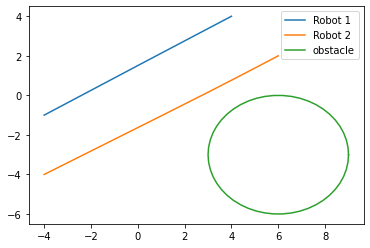
\includegraphics[width=10cm]{Graphs/Plot 1 parallel.png}
    \caption{Robot 1 travelling from (-4,-1) to (4,4) and robot 2 from (-4,-4) to (6,2) with obstacle centered at (6,-3) with a radius \( R = 3 \).}
    \label{fig:my_label}
\end{figure}

\begin{figure}[H]
    \centering
    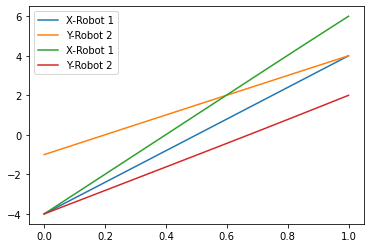
\includegraphics[width=10cm]{Graphs/Collsion free path for plot 1.png}
    \caption{Collision free path from figure 1}
    \label{fig:my_label}
\end{figure}

\begin{figure}[H]
    \centering
    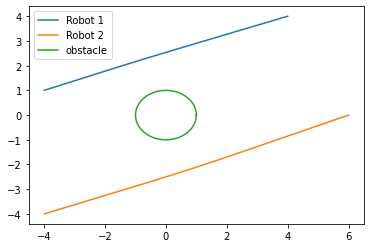
\includegraphics[width=10cm]{Graphs/Plot 2.png}
    \caption{Robot 1 with position (-4,1) at \( t = 0 \) and position (4,4) at \( t = 1 \) and robot 2 with a position at (-4,-4) at \( t = 0 \) and position (6,0) at \( t = 1 \). Obstacle centered at  (0,0) with radius \( R = 1 \).}
    \label{fig:my_label}
\end{figure}

\begin{figure}[H]
    \centering
    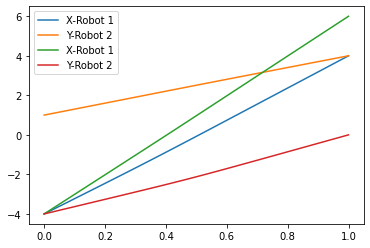
\includegraphics[width=10cm]{Graphs/Collision free path for plot 2.png}
    \caption{Collision free path from figure 3}
    \label{fig:my_label}
\end{figure}

\begin{figure}[H]
    \centering
    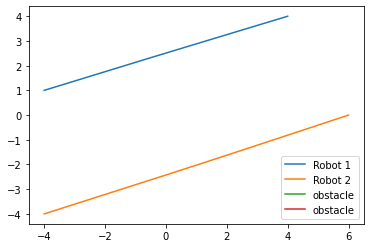
\includegraphics[width=10cm]{Graphs/Plot 3.png}
    \caption{Robot 1 with position (-4,1) at \( t = 0 \) and position (4,4) at \( t = 1 \) and robot 2 with a position at (-4,4) at \( t = 0 \) and position (6,0) at \( t = 1 \) with \textbf{no obstacle}.}
    \label{fig:my_label}
\end{figure}

\begin{figure}[H]
    \centering
    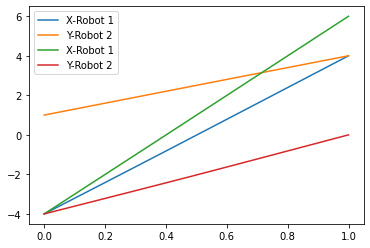
\includegraphics[width=10cm]{Graphs/Collision free path for plot 3.png}
    \caption{Collision free path from figure 5}
    \label{fig:my_label}
\end{figure}



\subsection{Two Robots With Paths That Intersect}


\begin{figure}[H]
    \centering
    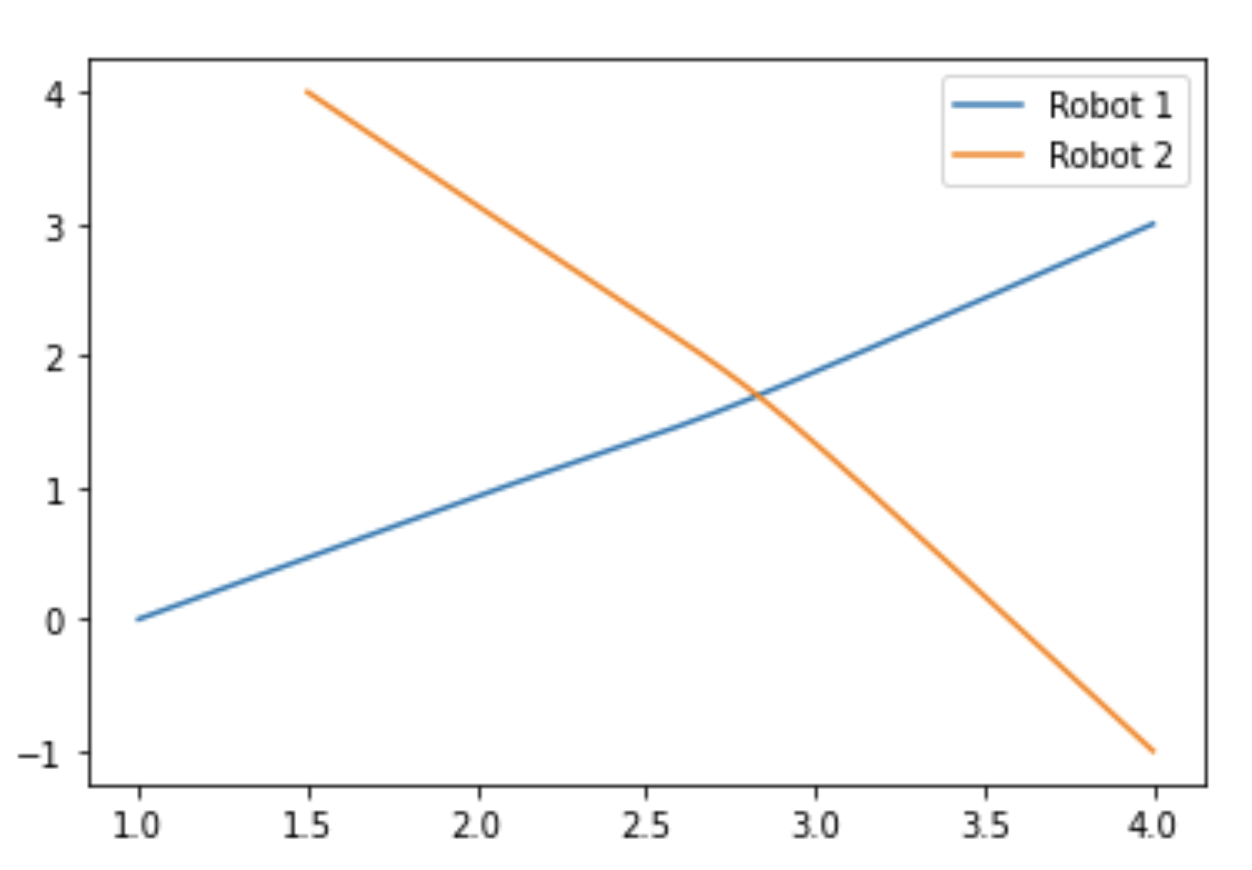
\includegraphics[width=10cm]{Graphs/Two Robots Intersecting (1).png}
    \caption{Robot 1 with position (1,0) at t = 0 and position (4,3) at t = 1 and robot 2 with position at (4,-1) at t = 0 and position (1.5,4) at t = 1 with \textbf{no obstacle}.}
    \label{fig:my_label}
\end{figure}


\subsection{Two Robots With Paths That Intersect}


\begin{figure}[H]
    \centering
    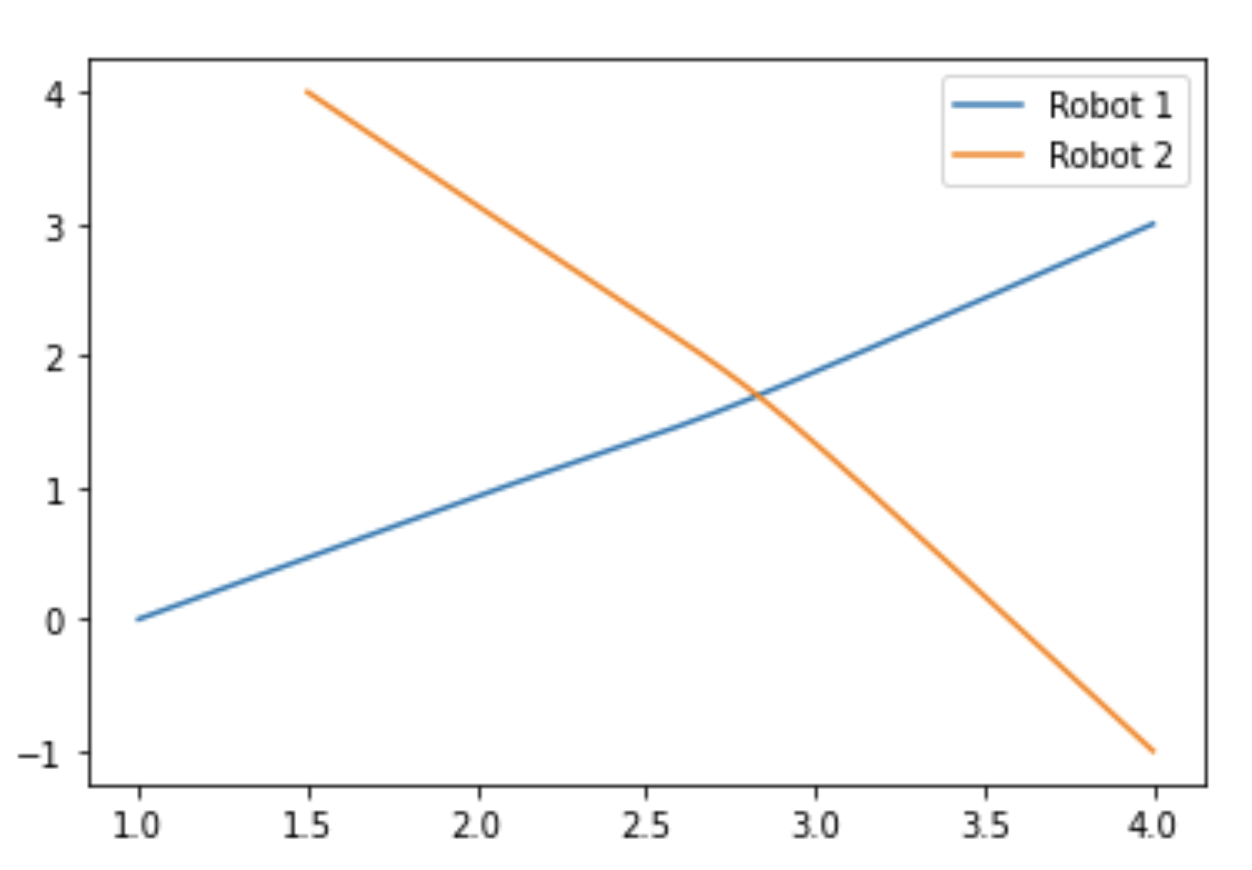
\includegraphics[width=10cm]{Graphs/Two Robots Intersecting (1).png}
    \caption{Robot 1 with position (1,0) at t = 0 and position (4,3) at t = 1 and robot 2 with position at (4,-1) at t = 0 and position (1.5,4) at t = 1 with \textbf{no obstacle}.}
    \label{fig:my_label}
\end{figure}




\begin{figure}[H]
    \centering
    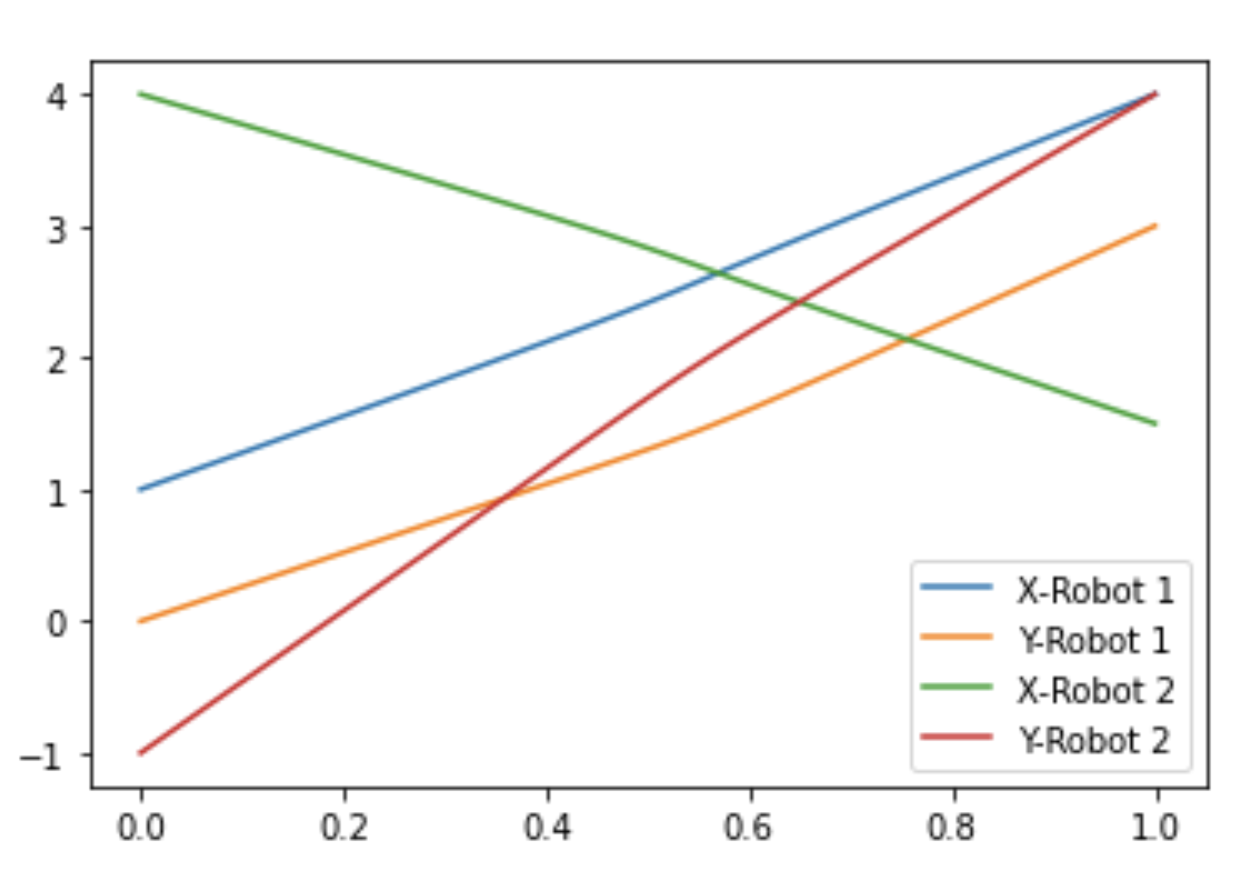
\includegraphics[width=10cm]{Graphs/Two Robots Intersecting (2).png}
    \caption{Collision free plot}
    \label{fig:my_label}
\end{figure}




\subsection{Two Robots And One Obstacle}


\begin{figure}[H]
    \centering
    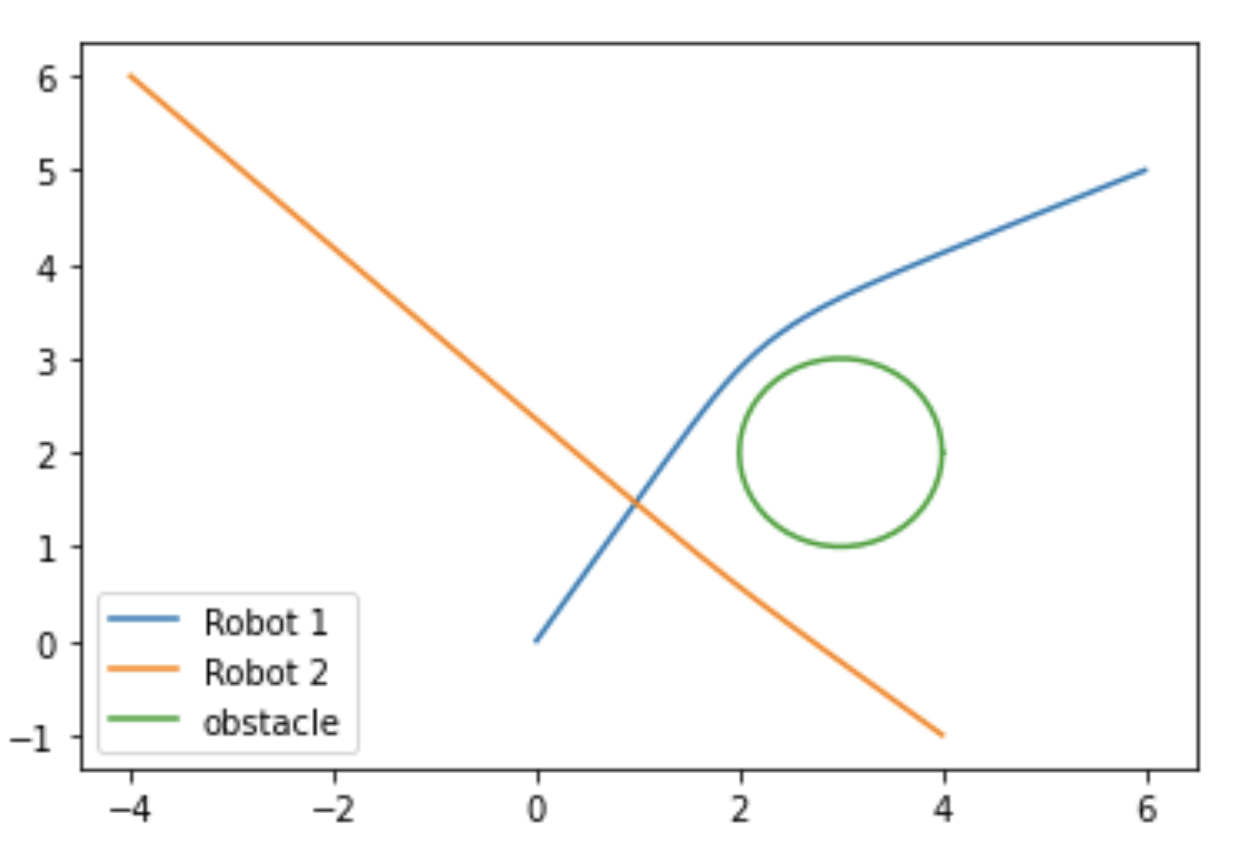
\includegraphics[width=10cm]{Graphs/2robots1obstacle.png}
    \caption{Robot 1 with position (0,0) at \( t = 0 \) and position (4,4) at \( t = 1 \) and robot 2 with a position at (4,-1) at \( t = 0 \) and position (0,4) at \( t = 1 \). Obstacle centered at (2,2) with radius \( R = 2 \).}
    \label{fig:my_label}
\end{figure}


\begin{figure}[H]
    \centering
    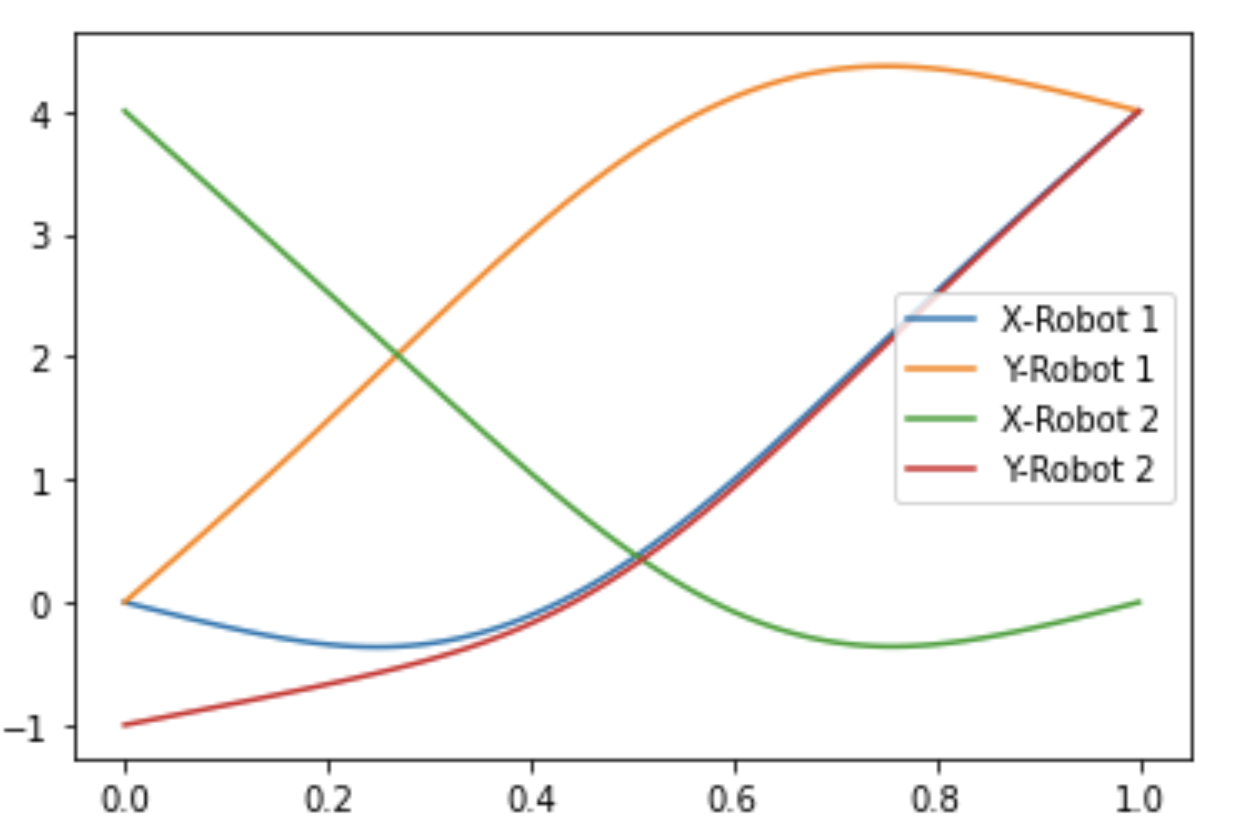
\includegraphics[width=10cm]{Graphs/collisionfree.png}
    \caption{Collision free plot of 7}
    \label{fig:my_label}
\end{figure}




\begin{figure}[H]
    \centering
    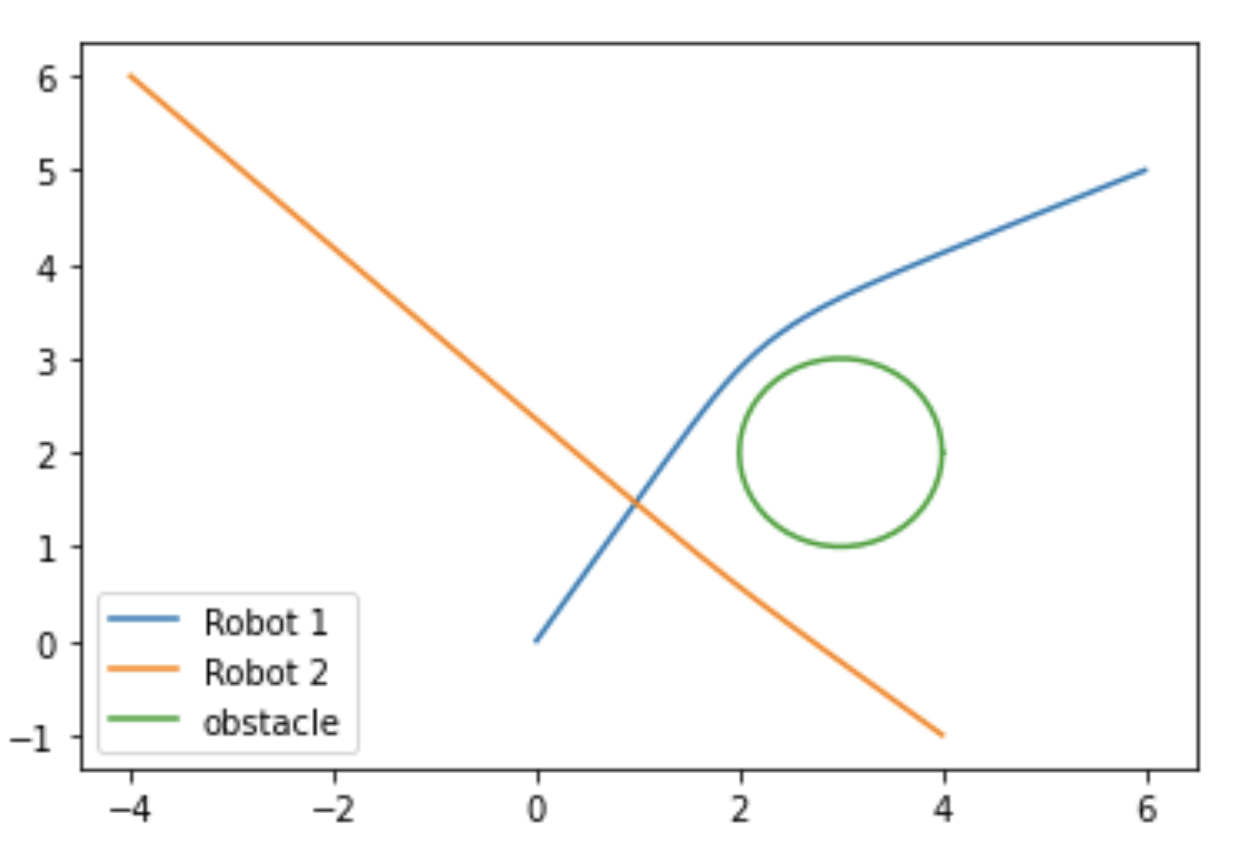
\includegraphics[width=10cm]{Graphs/2robots1obstacle.png}
    \caption{Robot 1 with position (0,0) at \( t = 0 \) and position (6,5) at \( t = 1 \) and robot 2 with a position at (4,-1) at \( t = 0 \) and position (-4,6) at \( t = 1 \). Obstacle centered at (3,2) with radius \( R = 1 \).}
    \label{fig:my_label}
\end{figure}






\begin{figure}[H]
    \centering
    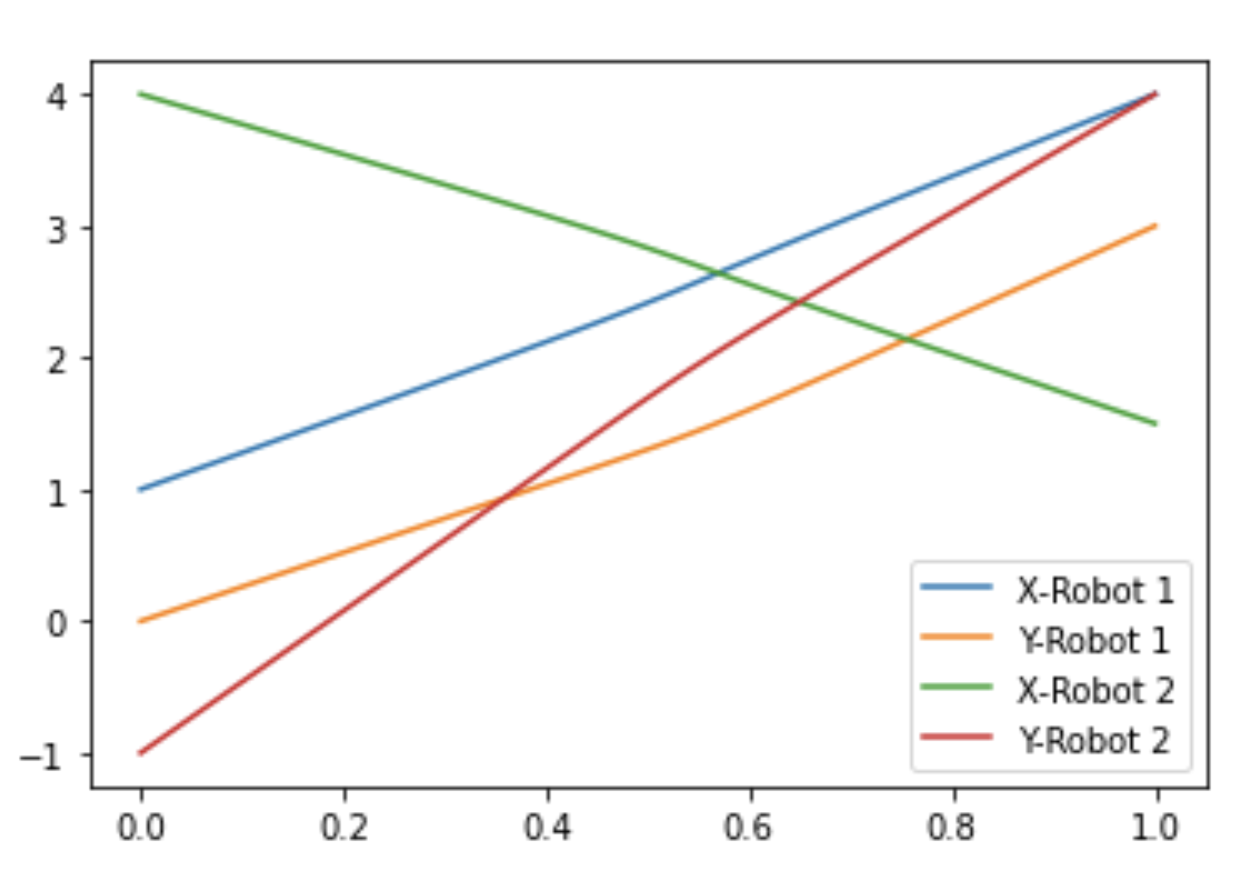
\includegraphics[width=10cm]{Graphs/Two Robots Intersecting (2).png}
    \caption{Collision free plot of figure 11} 
    \label{fig:my_label}
\end{figure}




\begin{figure}[H]
    \centering
    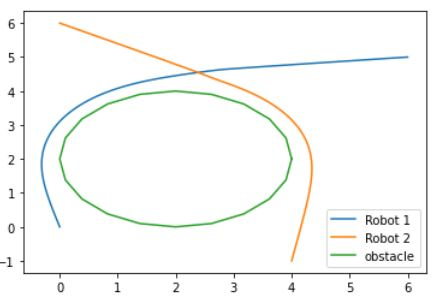
\includegraphics[width=10cm]{Graphs/plot for two robots and one obstacle.JPG}
    \caption{Robot 1 with position (-4,6) at \( t = 0 \) and position (6,5) at \( t = 1 \) and robot 2 with a position at (-4,6) at \( t = 0 \) and position (4,-1) at \( t = 1 \). Obstacle centered at  (2,2) with radius \( R = 2 \).}
    \label{fig:my_label}
\end{figure}

\begin{figure}[H]
    \centering
    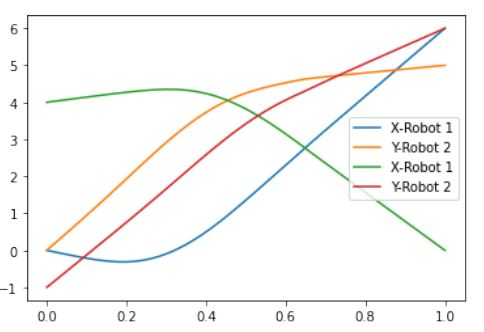
\includegraphics[width=10cm]{Graphs/Two Robots intersecting (3).JPG}
    \caption{Collision free plot of figure 13}
    \label{fig:my_label}
\end{figure}

